\subsection{Workflow Construction}

The workflow was constructed in four major stages.

\paragraph{Stage 1: phenotype cleaning.}
Phenotype processing was performed first because the entire modeling problem is antibiotic-specific. The cleaning sequence kept only rows belonging to isolates that also existed in the genotype table, retained only rows with the required identifying and label fields, restricted labels to \texttt{resistant} and \texttt{susceptible}, removed \texttt{(BioSample, Antibiotic)} pairs that contained both labels, and then resolved the remaining duplicate rows by selecting the lowest MIC after explicit ordering of the measurement sign.

After cleaning, antibiotics were retained only if they had at least 500 rows overall and at least 100 isolates in each class.

\paragraph{Stage 2: genotype cleaning and collapse.}
Genotype processing began from determinant-level records. Exact duplicate rows were removed first. The more difficult step was resolving repeated detections of the same determinant in the same isolate. To avoid counting one determinant multiple times, the table was collapsed to one row per \texttt{(BioSample, Element symbol)}.

When multiple rows competed for the same isolate-determinant combination, the preferred record was chosen using an explicit method-priority hierarchy: \texttt{EXACT}, \texttt{ALLELE}, \texttt{BLAST}, \texttt{POINT}, \texttt{PARTIAL}, \texttt{PARTIAL\_CONTIG\_END}, and finally \texttt{HMM}.

Remaining ties were broken by subtype-aware \texttt{P}/\texttt{X} preference, then by higher coverage and higher identity. This ensured that the final retained row for each determinant was biologically stronger and prevented repeated reporting from inflating the feature space.

\paragraph{Stage 3: class and subclass normalization.}
The raw genotype \texttt{Class} and \texttt{Subclass} fields were not directly usable because they often contained combined values. Typical cases included one class with multiple subclasses, multiple classes with multiple subclasses, \texttt{MULTIDRUG}, and rare subclass tokens that did not map cleanly from observed data alone.

Normalization therefore lower-cased class and subclass labels, split combined subclass strings into separate normalized rows, split combined class strings and reassigned subclass tokens using a registry built from simpler single-class observations, used the antibiotic grouping reference as additional guidance, and fell back to \texttt{unknown} only when no reliable assignment could be made.

Several biologically meaningful edge cases required explicit manual support before the \texttt{unknown} fallback. In particular, rifampin was mapped to rifamycin, clindamycin was mapped to lincosamide, and the combination drug trimethoprim-sulfamethoxazole was decomposed into trimethoprim and sulfonamide.

This normalization stage produced the final single-class, single-subclass genotype table used for connection.

\paragraph{Stage 4: genotype-to-phenotype connection and model-ready tables.}
For each eligible phenotype antibiotic, genotype evidence was connected back to the phenotype table under one of three scopes. The \textbf{strict} scope kept genotype rows whose normalized subclass matched the narrow lineage token set of the target antibiotic. The \textbf{broad} scope kept genotype rows whose normalized class matched the broader allowed class set of the target antibiotic. The \textbf{all} scope kept every normalized genotype row observed for the isolates in that antibiotic-specific phenotype table.

\begin{figure}[!htbp]
\centering
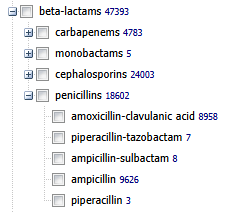
\includegraphics[width=0.45\textwidth]{figures/scope_broad_example}
\caption[Broad-scope hierarchy example.]{Illustrative broad-scope hierarchy for beta-lactam antibiotics.}
\label{fig:broad-scope-example}
\end{figure}

Once scope matching was applied, genotype rows were aggregated by isolate and determinant, then pivoted into wide antibiotic-specific model-input tables containing determinant coverage, determinant identity, and lineage-match features.

\begin{figure}[!htbp]
\centering
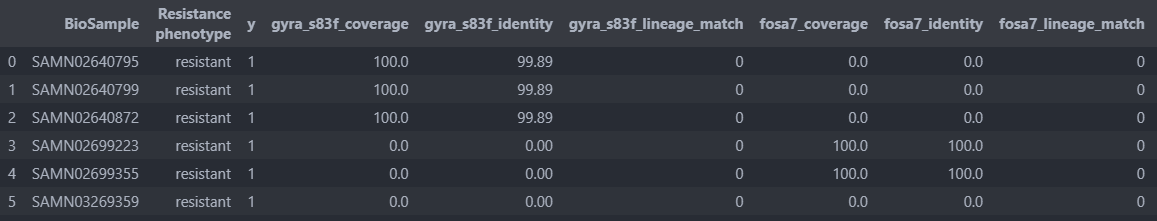
\includegraphics[width=0.85\textwidth]{figures/prepared_input_example}
\caption[Prepared model-input example.]{Example of a prepared model-input table after genotype evidence has been aligned with phenotype labels.}
\label{fig:prepared-input-example}
\end{figure}

This staged construction is what made the later comparison scientifically meaningful: model differences could be interpreted relative to explicit decisions about phenotype cleaning, determinant normalization, and biological connection scope.
